%%%%%%%%%%%%%%%%%%%%%%%%%%%%%%%%%%%%%%%%%
% University Assignment Title Page 
% LaTeX Template
% Version 1.0 (27/12/12)
%
% This template has been downloaded from:
% http://www.LaTeXTemplates.com
%
% Original author:
% WikiBooks (http://en.wikibooks.org/wiki/LaTeX/Title_Creation)
%
% License:
% CC BY-NC-SA 3.0 (http://creativecommons.org/licenses/by-nc-sa/3.0/)
% 
% Instructions for using this template:
% This title page is capable of being compiled as is. This is not useful for 
% including it in another document. To do this, you have two options: 
%
% 1) Copy/paste everything between \begin{document} and \end{document} 
% starting at \begin{titlepage} and paste this into another LaTeX file where you 
% want your title page.
% OR
% 2) Remove everything outside the \begin{titlepage} and \end{titlepage} and 
% move this file to the same directory as the LaTeX file you wish to add it to. 
% Then add \input{./title_page_1.tex} to your LaTeX file where you want your
% title page.
%
%%%%%%%%%%%%%%%%%%%%%%%%%%%%%%%%%%%%%%%%%
%\title{Title page with logo}
%----------------------------------------------------------------------------------------
%	PACKAGES AND OTHER DOCUMENT CONFIGURATIONS
%----------------------------------------------------------------------------------------

\documentclass[a4paper, 12pt]{article}

\usepackage[utf8]{inputenc}
\usepackage[T1]{fontenc}
\usepackage[french]{babel}
\usepackage{amsmath}
\usepackage{graphicx}
\usepackage[colorinlistoftodos]{todonotes}

\DeclareUnicodeCharacter{202F}{\,} 

\usepackage{enumitem}
%\usepackage[dvipsnames]{xcolor}
\usepackage{csquotes}
\usepackage[hypcap=false, font={small}, labelfont=bf]{caption} % image caption configuration

\usepackage[breaklinks]{hyperref} % breaking links
\hypersetup{
	colorlinks=true
	linkcolor=black
	urlcolor=NavyBlue
}

\frenchbsetup{StandardLists=true}

%\setlength{\parindent}{0cm}

%=================================
% Color definition section
%=================================
\definecolor{listGreen}{HTML}{4dffb5}
\definecolor{listGrey}{HTML}{BBBCEE}
\definecolor{listLightGrey}{HTML}{DDDDFF}

% redefining vertical spaces
\newcommand\vertspace{\vspace{0.50cm}}

% cross-referencing words 
\makeatletter
\newcommand{\setword}[2]{%
  \phantomsection
  #1\def\@currentlabel{\unexpanded{#1}}\label{#2}%
}
\makeatother

\begin{document}

\begin{titlepage}

\newcommand{\HRule}{\rule{\linewidth}{0.5mm}} % Defines a new command for the horizontal lines, change thickness here

\center % Center everything on the page
 
%----------------------------------------------------------------------------------------
%	HEADING SECTIONS
%----------------------------------------------------------------------------------------

\textsc{\LARGE Gestion des données \& Business Intelligence }\\[0.4cm] % Name of your university/college
%\textsc{\LARGE INSTITUTE OF TECHNOLOGY  }\\[0.3cm]
\textsc{\Large Expertise Informatique et système d'information}\\[0.5cm] % Major heading such as course name
 % Minor heading such as course title

%----------------------------------------------------------------------------------------
%	TITLE SECTION
%----------------------------------------------------------------------------------------

\HRule \\[0.4cm]
{ \huge \bfseries Conception, modélisation \& \\implantation d'une solution B.I}\\[0.03cm] % Title of your document
\HRule \\[1.5cm]

 
%----------------------------------------------------------------------------------------
%	AUTHOR SECTION
%----------------------------------------------------------------------------------------

\begin{minipage}{0.4\textwidth}
\begin{flushleft} \large
\emph{Soumis par:}\\
Jimmy BOUMANS \\Mathieu DORVILLE\\Florian GAUTIER\\Jérémie LAERA\\Arthur TOULOUMOND % Your name
\end{flushleft}
\end{minipage}
~
\begin{minipage}{0.4\textwidth}
\begin{flushright} \large
\emph{Destiné à:} \\
EPSI Bordeaux % Supervisor's Name
\end{flushright}
\end{minipage}\\[1cm]

% If you don't want a supervisor, uncomment the two lines below and remove the section above
%\Large \emph{Author:}\\
%John \textsc{Smith}\\[3cm] % Your name

%----------------------------------------------------------------------------------------
%	DATE SECTION
%----------------------------------------------------------------------------------------

{\large Année universitaire 2020-2021} % Date, change the \today to a set date if you want to be precise

%----------------------------------------------------------------------------------------
%	LOGO SECTION
%----------------------------------------------------------------------------------------


\includegraphics[scale=0.16]{images/epsi_logo.jpg}\\[1cm] % Include a department/university logo - this will require the graphicx package
 
%----------------------------------------------------------------------------------------

\vfill % Fill the rest of the page with whitespace

\end{titlepage}




\newpage
\tableofcontents
\newpage





\section{Introduction \& Contexte}

La direction de SO-EMBALLAGE est décidée à lancer un projet de grande envergure. Au vu des réflexions déjà menées par les différents responsables des services, il apparaît que l’organisation toute entière devra sans doute subir quelques modifications. Il en suivra une refonte complète du système d’information.

Son besoin est concentré sur la nécessité de rester un acteur important dans le domaie de l'emballage, c'est pourquoi SO-EMBALLAGE souhaite répondre à différentes problématique au travers des décisions suivantes.   

\begin{itemize}[label=\textbullet, font=\LARGE \color{listGreen}]	
	\item La mise en place d’outils pour une meilleure sélection des fournisseurs et de produits sur la base d’un ensemble de critères. 
	\item Une meilleure gestion des stocks pour moderniser son organisation et assurer un service clientèle de qualité. 
\end{itemize} 

C’est pourquoi notre équipe intervient dans l’accompagnement de SO-EMBALLAGE et propose au travers de ce dossier une première solution ainsi que des recommandations pour y arriver.    

Nous allons par l'intermédiaire de cet écrit vous décrire et présenter notre ébauche de réalisation.    


\newpage

\section{Conception d'un Data Warehouse ou Datamart}

\subsection{Étude des données produites par l’intermédiaire des applications actuellement en place}

%Lorsque nous étudions la base de données existante nous pouvons constater les éléments suivants :  
%\begin{itemize}[label=\textbullet, font=\LARGE \color{listGreen}]	
	%\item Les tables suivantes inutilisées : LIVRAISON$\_$C / DETAIL$\_$LIVR$\_$C / MOUVEMENT$\_$STOCK 
	%\item Les tables Client et Fournisseur sont séparables en tables Adresse et Contact 
	%\item Il n’y a pas d’indication de capacité de stockage des hangars 
	%\item La table Emplacement est séparable en tables Hangars et Site : 
	%\begin{itemize}[label=\textbullet, font=\LARGE\color{listGrey}]
		%\item Hangar : adresse capacité type de stockage (produit humide etc.) 
		%\item Emplacement : Allée Rayon capacité en m3 
	%\end{itemize}
	%\item Pour la table « Achat » :
   %\begin{itemize}[label=\textbullet, font=\LARGE\color{listGrey}]
		%\item Le champ « comment_achat » contient des informations résumables en ENUM
		%\begin{itemize}[label=\textbullet, font=\LARGE\color{listGrey}]
			%\item Urgent
			%\item Opération promotionnelle 
			%\item Normal
		%\end{itemize}
	%\end{itemize}	 	
%\end{itemize}

Le point suivant résume notre analyse primaire sur le modèle de données de SO-EMBALLAGE. Un résumé synthétique est disponible dans la section \ref{Résumé} en fin de section.  \vertspace 


Lorsque nous étudions la base de données existante nous pouvons constater les éléments suivants :  

\begin{itemize}

	\item Les tables suivantes inutilisées : LIVRAISON$\_$C / DETAIL$\_$LIVR$\_$C / MOUVEMENT$\_$STOCK
	\item  Les tables \textit{Client} et \textit{Fournisseur} sont séparables en tables \textit{Adresse} et \textit{Contact}  
	\item Il n’y a pas d’indication de capacité de stockage des hangars  \vertspace 
	\item La table \textit{Emplacement} est séparable en tables \textit{Hangars} et \textit{Site} :  


		\begin{itemize}
		
			\item Hangar : adresse, capacité, type de stockage (produit humide etc.)   

 			\item Emplacement : Allée, Rayon, capacité en m$^3$		
		
		\end{itemize} 

	\item Pour la table \textit{Achat} :  
	
		\begin{itemize}
			\item Le champ \textit{comment$\_$achat} contient des informations résumables en ENUM   
		

				\begin{itemize}

					\item Urgent
					\item Opération promotionnelle 
					\item Normal
				\end{itemize}
				
		\end{itemize}
	 
	\item Dans la table \textit{Produit}  

		\begin{itemize}
		  \item Il y a un manque d’informations sur le conditionnement : 
			 
			\begin{itemize}

				\item Quel volume prend un lot ? 
				\item Conditionner par lot ou à l’unité 
	
			\end{itemize}
		

			\item Il n’y a pas d’indication de taille, uniquement à l’unité 

			\item L’indication de quantité par lot est contenue dans un champ texte libre (comment$\_$produit) 	
		\end{itemize}	
	
	\item Aucun suivi des pertes dégradation ou vol 

	\item Aucun lien entre ce qui a été livré et commandé 

	\item La table \textit{mouvement stock} peut sembler inutile (non-alimentée et non-utilisée)
	
\end{itemize}	

\vertspace 
	
Afin de pouvoir définir les changements à appliqués aux SGBD il est bon de rappeler les besoins de l’entreprise :   

Les besoins principaux relevés sont les suivants :

\begin{itemize}

	\item - Évitez le surstock/sous-stock 

	\item Prédire les effets de mode 

	\item Évitez les livraisons partielles 

   \item Évitez le blocage de l’activité 

\end{itemize}  

\vertspace


	
Afin de pouvoir identifier les points de blocages et de répondre au mieux aux besoins nous devons évaluer les performances de fonctionnement de l’entrepôt. Ces performances peuvent être mesurées à l’aide d’indicateurs. Certains d'entre eux dépendent de données de la SGBD. En identifiant ces indicateurs nous pourrons déduire les données manquantes dans le SGBD d'origine. 

\vertspace 

Afin d’éviter le surstock/sous-stock , nous souhaitons parcourir les axes suivants dans les prochaines sous-sections.  	  

\subsubsection{Calcul de la méthode Wilson}  

\begin{itemize}
	\item Permet de déterminé la quantité optimale pour un réassort 

	\item Calcul les délais optimaux entre chaque de commande 

	\item Optimise les coûts de stock 

	\item Optimise les coûts de passage de commande 
	
	\begin{itemize}
		\item Limites :
			\begin{itemize}
			
				\item Fonctionne mal pour une demande instable 

				\item Fonctionne mal avec des délais inconstants ou imprévisibles 			
			
			\end{itemize}
		\end{itemize}				 

	\begin{itemize}
		\item Données : 

			\begin{itemize}

				\item Coût de passage de la commande : 
	
					\begin{itemize}
						\item Comporte le prix HT de la ressource à rajouter dans la table Achat 

						\item Charges transporteur
					\end{itemize}
				
				\item Le coût de stock 

				\item La demande pour ce produit 
				
	\end{itemize}
	
	\end{itemize}
	
\end{itemize}





\subsubsection{Optimisation du stock de sécurité :}  

\begin{itemize}
	\item Complète la méthode de Wilson 

	\item Permet de couvrir la demande incertaine 

	\item Permet de couvrir les délais incertains 

	\item Plusieurs méthodes de calcul à adapter en fonctions des besoins 
\end{itemize}

\begin{itemize}
	\item Données :
	
	\begin{itemize}
		\item Les ventes pour un produit représenté par la somme des détails commande 
	\end{itemize}
		  
\end{itemize}


\subsubsection{Taux de disponibilité : mesure quelle quantité de nos produits sont en vente} 

\begin{itemize}

	\item Données :  produits/quantité  

	\item Calcul :
	
		\begin{itemize}
			\item Pour chaque produit en stock : 
			
				\begin{itemize}
					\item Disponibilité : Si quantité > 0 = 100\% 				
				\end{itemize}
				
			\item Faire la moyenne : Somme disponibilité / nombre produits 	
		\end{itemize}	  

\end{itemize} 

\subsubsection{Taux d’occupation : mesure la place disponible dans les hangars} 

\begin{itemize}

	\item Calcul : Place occupée / place total 
	
	\item Données : 
	
	\begin{itemize}
	
		\item Somme de la capacité de tous les emplacements d’un même hangar  
		
		\item Données de volume des produits/conditionner 
		
	\end{itemize}

\end{itemize}

\vertspace

\subsubsection{Prédire les effets de mode}

\begin{itemize}

	\item Fiabilité de la prévision: Permet de d’ajuster et d’anticiper la mobilisation de moyens et de ressources. Nous pourrons en déduire par produits la quantité moyenne consommée et les pics de consommation, afin d’en produire un lot minimum de fonctionnement. 
	
		\begin{itemize}
		
			\item Calcul : 
			
				\begin{itemize}
				
					\item Définir une période  

					\item Pour chaque article 

					\item Calculer l’écart absolu entre la vente réelle et la vente effectuée 

					\item Diviser par la vente réelle 

					\item Prendre le résultat et le soustraire à 1 

					\item Faire le pourcentage de toutes les prévisions 				
				
				\end{itemize}						
		
		\end{itemize}

\end{itemize}


\subsubsection{Eviter les livraisons partielles} 

\begin{itemize}


	\item Taux de service :  Permet de mesurer notre capacité à livrer, et d’évaluer nos prestataires de livraisons.  Deux informations peuvent être extraites. 
	
		\begin{itemize}
		
			\item Calcul:  
			
				\begin{itemize}
				
					\item Récupérez la liste complète des commandes reçues sur la période souhaitée 

					\item Récupérez ensuite sur ces même articles le nombre de commandes livrées dans les temps. Si celles-ci sont en retard, alors entrez 0%  

					\item Divisez les commandes livrées par les commandes reçues pour connaitre votre taux de service. 
				
				
				\end{itemize}		
								
			\item Données : 
				
				\begin{itemize}
				
					\item Commande/date 

					\item Details$\_$Commande/quantité 

					\item Livraison/date$\_$départ 

					\item Livraison/date$\_$arrivée 

					\item Livraison/date$\_$estimée 

					\item Coût livraison 

					\item Details$\_$Livraison/quantité 

					\item Livreur
					
						\begin{itemize}
						
							\item  Permet d’identifier quel transporteur auxquelles nous avons fait appel pour cette livraison. 						
						
						\end{itemize}						  				
				
				\end{itemize}
		
		\end{itemize}

\end{itemize} 

\vertspace

\subsubsection{Evitez le blocage de l’activité}

\begin{itemize}

	\item Livraison dans les temps :  
	
		\begin{itemize}
		
			\item Permet d’identifier les retards et leur raisons 

			\item Calcul de pourcentage entre livraison respecté sur livraison total 

			\item Calcul de pourcentage entre livraison en retard sur livraison total 		
			
				\begin{itemize}
				
					\item Pourcentage d’une raison du retard sur le total de livraison retard 				
				
				\end{itemize}
				
			\item Données : 
			
				\begin{itemize}
					
					\item Livraison/date$\_$départ 

					\item Livraison/date$\_$arrivée 

					\item Raison du retard 					
					
				\end{itemize}					
		
		\end{itemize}
		
	\item Rotation de stock : Permet de mesurer en combien de temps met votre stock à s’épuiser. 
	
		\begin{itemize}
		
			\item  Calcul : 
			
				\begin{itemize}
				
					\item Déterminé une période 

					\item Stock moyen : Moyenne de produit vendu sur cette période 

					\item Calculer la valeur HT du stock moyen 

					\item Multiplier le nombre de vente total par le nombre de jour de la période 

					\item Diviser la valeur du stock moyen par le résultat de la multiplication 				
				
				\end{itemize}
				
			\item Données  
			
				\begin{itemize}
				
					\item Commande détails / Quantité  				
				
				\end{itemize}											
		
		\end{itemize}			
		
	\item Taux de démarque : Permet de calculer le nombre de perte/vol/remise etc...
	
		\begin{itemize}
	
			\item Calcul : 
			
				\begin{itemize}
				
					\item Valeur stock après inventaire / Valeur du stock théorique $\times$ 100 				
				
				\end{itemize}				 	
				
			\item Données :   
			
				\begin{itemize}
				
					\item Somme de ( Produit Quantité $\times$ Prix HT )  

					\item Somme de ( Produit Compté $\times$ Prix HT)
					
						\begin{itemize}
						
							\item Table \textit{Inventaire} : champs quantité et date$\_$inventaire						 						
						
						\end{itemize}						  				
				
				\end{itemize}					
	
		\end{itemize}
		
	\item Coût logistique et transport: Représente la part de la logistique et du transport sur le CA , exprimé en pourcentage du chiffre d’affaire total(1). Représente également le coût moyen par article du coût de la logistique et du transport, exprimé en pourcentage du chiffre d’affaire total(2). 
	
		\begin{itemize}
		
			\item Calcul :  
			
				\begin{itemize}
				
					\item Sur l’année : (cout total d’entreposage + Coût total des transporteurs + Charge de service) / CA $\times$ 100 	(1)			
					\item Sur l’année : (cout total d’entreposage + Coût total des transporteurs + Charge de service) /Valeur total de la marchandise vendu $\times$ 100 
				\end{itemize}						
		
		\end{itemize}
	

\end{itemize}

\vertspace  
% ===========================================

\subsubsection{Résumé des analyses préalables} \label{Résumé}

Pour résumé les changements supplémentaires à apporter aux SGBD : 


%============================================

\begin{itemize}[label=\textbullet, font=\LARGE \color{listGreen}]	


\item Table \textit{Produit} : 

	\begin{itemize}[label=\textbullet, font=\LARGE \color{listGrey}]	
		\item Il n’y a pas de distinction de quantité entre ce qui est disponible et ce qui attend d’être livré 

		\begin{itemize}[label=\textbullet, font=\LARGE\color{listLightGrey}]
			\item Ajout Quantité en stock 

	   		\item Ajout Quantité disponible 
		\end{itemize}


	\item Ajout Poids 

	\item Ajout Quantité$\_$lot 

	\item Possède 0 ou plusieurs inventaires 

	\item Possède 0 ou plusieurs conditionnements 
	\end{itemize}


\item Création Table \textit{Inventaire} : 

	\begin{itemize}[label=\textbullet, font=\LARGE \color{listGrey}]
		\item Quantité  

		\item Date 
	\end{itemize}


\item Création table \textit{Conditionnement} :  

	\begin{itemize}[label=\textbullet, font=\LARGE \color{listGrey}]
		\item Largeur 

		\item Hauteur 

		\item Longueur 

		\item Poids 

		\item Quantité 
	\end{itemize}


\item Table \textit{Emplacement} : 

	\begin{itemize}[label=\textbullet, font=\LARGE \color{listGrey}]
		\item Possède 1 hangar 

		\item Ajout Espace$\_$disponible$\_$m$^3$ 

		\item Ajout Rayon
	\end{itemize}
 

\item Table \textit{Livraisons} :  

	\begin{itemize}[label=\textbullet, font=\LARGE \color{listGrey}]
		\item date$\_$départ 

		\item date$\_$arrivée 

       \item date$\_$estimée 
	
		\item Coût livraison 

		\item A obligatoirement un Transporteur 
	\end{itemize}


\item Création Table \textit{Transporteur} 

	\begin{itemize}[label=\textbullet, font=\LARGE \color{listGrey}]
		\item Nom 

		\item Délai vendu 
	
		\item Garantie
	\end{itemize}
 

\item Création table énumération \textit{Origine du retard} : 

	\begin{itemize}[label=\textbullet, font=\LARGE \color{listGrey}]
		\item Délai non respecté par le fournisseur 

		\item Délai non respecté par le transporteur 

		\item Erreur de stock 

		\item Qualité  

		\item Regroupement pour expédition 
	\end{itemize}


\item Table Detail$\_$achat : 

	\begin{itemize}[label=\textbullet, font=\LARGE \color{listGrey}]
		\item Indiquez le prix de l’unité acheté en HT 
	\end{itemize}


\end{itemize}

   

\subsection{Étude des données provenant de sources externes}  

Notre recherche de types de données externes nous a conduit à trouver les sources de données suivantes :  

\begin{itemize}[label=\textbullet, font=\LARGE \color{listGreen}]	
    \item \textbf{PackPlus} (\url{https://www.packplus.in/}) : Propose une newsletter tous les 15 jours avec des informations sur le monde de l’emballage (Ces données sont à exploiter manuellement puisqu’il d’une newsletter avec des statistiques, des tendances de marchés et des actualités).
	\item \textbf{Japan Packaging Institute (JPI)} (\url{https://www.jpi.or.jp/english/}) : Le JPI propose énormément d’informations intéressantes puisqu’il intervient dans les domaines suivants :   
	\begin{itemize}[label=\textbullet, font=\LARGE \color{listGrey}]	
		\item Réalisation d'enquêtes et de travaux de R\&D liés à l'emballage 
		\item Collecte de données relatives au conditionnement, à la production de statistiques, etc. et partage de ces informations 
		\item Développement de concepts d'emballages
		\item Éducation sur l'emballage et formation du personnel 
		\item Consultation et orientation concernant les emballages  
		\item Création et promulgation de normes d'emballage, et conduite d'activités éducatives à leur intention au Japon et à l'étranger 
		\item Échange d'informations et collaboration avec des organisations liées à l'emballage au Japon et à l'étranger 
		\item Mener des activités mondiales liées à l'emballage, organiser des expositions sur l'emballage  
		\item Publication et vente de livres sur l'emballage. 
	\end{itemize}
	Il existe un onglet statistique regroupant énormément d’informations sur le domaine de l’emballage, ainsi qu’une section regroupant les dernières publications sur ce domaine.
	\item\textbf{ L’université du Michigan} (\url{https://www.canr.msu.edu/packaging/research/}) : L’université dispose d’un centre de recherche sur le packaging. La périodicité de parution des données est aléatoire mais reste une bonne source de d’informations. 
	\item \textbf{Transparency Market Research} (\url{https://www.transparencymarketresearch.com/packaging-market-reports-35.html?page=2}) : Il s’agit d’un site internet qui regroupe énormément d’études axés sur le domaine de l’emballage. Il est possible d’y retrouver des graphes, des tableaux, des statistiques, des indicateurs d’opportunités ou menaces… Il est cependant important de signaler que cette source de données est payante, cela signifie donc un investissement de la part de SO-EMBALLAGE. 
	\item \textbf{Syskevasia} (\url{https://syskevasia-expo.gr/en/}) est une société Grecque axée sur les expositions ayant pour but de promouvoir les techniques les plus actuelles en matière d’emballage de tout type. “Packaging at its best” comme l’indique son slogan accrocheur, la société se veut innovatrice et convie chaque année divers entreprises spécialisées dans la production d’emballage par le biais d’expositions. Plus d’information sont disponibles sur le site officiel, traduit en anglais depuis la langue grecque.  
\end{itemize}

L’extraction, l’uniformisation, l’analyse et l’exploitation de ces données nécessitent une intervention humaine. Bien-sûr, une partie de ces processus peuvent être automatisés mais la plupart, telle que la lecture des newsletters pour identifier les informations importantes, restent à la charge d’une personne. Il peut donc être intéressant pour la société SO-EMBALLAGE de former une personne en interne ou alors de recruter une personne disposant déjà des compétences nécessaires.   \vertspace

Conjointement aux possibilités multiples d’observer et de travailler avec les sources de données externes, SO-EMBALLAGE devrait orienter ses actions vers un recrutement spécifique. Les ressources possédant les compétences en lien à ces activités sont des ressources cruciales : développeur senior ou data scientist, il conviendra d’effectuer les choix nécessaires afin de s’adapter au nouveau projet imminent. Nous mentionnons le poste de data scientist car les masses de données que la société collecte peuvent devenir volumineuses et nécessiter des analyses mathématiques plus approfondies : nous souhaitons mettre en avant le domaine du Data Mining. 

\subsection{L’apport du Data Mining \& la visualisation des données de So Emballage}   

\textbf{Data Mining} signifie “exploration de données”. L’idée principale est de détecter des motifs, les visualiser en les explosant, les modéliser (normalisation, classification) et enfin de les expliquer. Il s’agit d’effectuer de la description à l’aide de statistiques descriptives dans le but de produire des résultats graphiques.  

Le cas de figure de la société française SO-EMBALLAGE par le biais de son désir d’implémenter une solution Business Intelligence apporte une problématique touchant le domaine du Data Mining.  Cependant, il ne faut pas mélanger BI et Data Mining, la dernière ne produisant pas de données de sortie.  Dans l’idéal, l’exploration des données de SO-EMBALLAGE pourrait subir l’ajout d’algorithmes de Machine Learning afin d’effectuer des prédictions.   

Exemple : Nous disposons de données telles que les quantités de produits disponibles ainsi que du nombre de commandes par mois. Nous avons donc dans un premier temps choisi de créer un affichage sur le nombre de produits restant pour chaque mois effectif. Ensuite, étant donné que nous possédons des données sur les commandes échelonnées sur plusieurs mois, nous recommanderions de mettre en place un système de prédiction afin d’avoir une visibilité sur les commandes pour les mois à venir. Ainsi l’entreprise et ses décisionnaires auraient une nouvelle force : ils pourraient revoir les stocks en fonction des résultats.  \vertspace

So Emballage pourrait tout d’abord avoir recours au modèle de processus \textbf{CRISP-DM (Cross Industry Standard Process for Data Mining)} \footnote{Conçu en 1996 et élue méthode la plus utilisée par les Data Miners depuis 2002.}. Il s’agit d’une approche séparant le processus de Data Mining en six étapes au sein d’un projet IT :  
 
\begin{itemize}[label=\textbullet, font=\LARGE \color{listGreen}]
	\item La compréhension du métier 
	\item La compréhension des données  
	\item La préparation des données 
	\item La modélisation des données 
	\item L’évaluation
	\item Le déploiement du produit 
\end{itemize}  

\begin{center}
	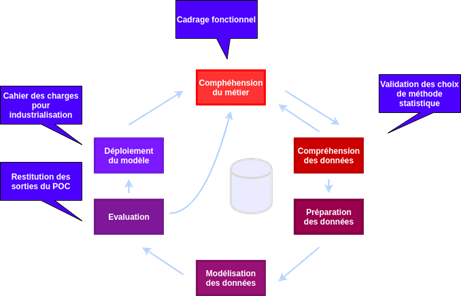
\includegraphics[scale=0.8]{images/data_mining_crispdm.png} 
	\captionof{figure}{La méthode CRISP-DM représentée pour un processus lambda au sein d'un projet informatique}
\end{center} 

Lors du recours à cette démarche, il convient d’établir une communication accentuée entre les experts en Data Mining et les ressources du métier.   \vertspace 

Actuellement, la solution que nous proposons utilise des composantes de ce domaine par le biais de l’outil Google Data Studio. D’autres solutions sont envisageables et nous les mentionnerons dans notre section dédiée à cet effet. 

\newpage

\section{Conception du Datamart afin de répondre à la problématique de l’entreprise SO-EMBALLAGE}  

Si nous reprenons le besoin initial, nous pouvons schématiser une première architecture permettant de visualiser ce vers quoi nous souhaitons nous orienter : 

\begin{center}
	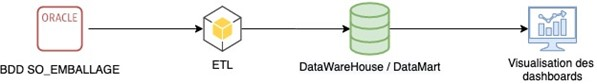
\includegraphics[scale=0.86]{images/solution_generale.jpg} 
	\captionof{figure}{Schéma de la solution générale pensée}
\end{center}  

Pour répondre à cette problématique nous sommes tout d’abord parti sur une solution moderne et innovante autour d’une technologie appelée « Suite Elastic ». Cette terminologie regroupe en réalité plusieurs outils dont trois en particulier qui s’avèrent très intéressant dans la situation de SO-EMBALLAGE :  

La conception d’un Datawarehouse peut être réalisée par le biais de trois modèles : 
\begin{itemize}[label=\textbullet, font=\LARGE \color{listGreen}]
	\item Elastic Search
	\item Logstash 
	\item Kibana 
\end{itemize} 

Il s'agit d'une suite fiable et sécurisée, qui vous permet de collecter n'importe quel format de données depuis n'importe quelle source, puis d'interroger, d'analyser et de visualiser vos données en temps réel.  

\begin{center}
	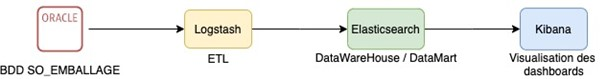
\includegraphics[scale=0.86]{images/solution.jpg} 
	\captionof{figure}{Schéma de la solution portant sur la suite ELK}
\end{center}  

Après une étude approfondie des impacts, du temps nécessaires à la mise en place d’une telle solution et de par sa complexité, nous n’avons pas souhaité conserver cette dernière (qui reste tout de même intéressante pour une mise en place à plus grande échelle). Dès lors, nous nous sommes orientés vers des solutions alternatives moins chronophage et qui nous permettent de vous présenter des solutions viables à vos problématiques. 

\subsection{Solution A}

Pour cette première solution, la base de données SO-EMBALLAGE est retravaillée en base de données MariaDB dans un souci de compétences techniques et de simplicité d'utilisation, ce qui signifie que si cela est nécessaire il est tout à fait possible de rester sur une base de données Oracle. Ensuite, un script javascript faisant office d’ETL permet d'extraire les données utiles pour notre situation, de faire des modifications dessus et de les ajouter dans une autre base de données MariaDB qui fait office de DataWarehouse. Enfin, nous utilisons un logiciel afin de visualiser sous forme de tableaux et graphiques les données de notre DataWarehouse, tel que Google Data Studio ou encore Microsoft Power BI \footnote{Power BI offre un panel de fonctionnalités gratuites ainsi qu'une version en ligne avec d'autres caractéristiques}. 

\begin{center}
	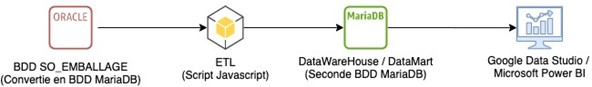
\includegraphics[scale=0.86]{images/solution_a.jpg} 
	\captionof{figure}{Schéma de la première solution proposée}
\end{center}  

\subsection{Solution B}

Une alternative à la première solution est d'oublier l'étape du script permettant d'extraire les données de notre première base de données, mais plutôt d'utiliser des vues SQL qui permettent d'obtenir les données voulues grâce à la bonne combinaison de requêtes. La différence réside dans le fait que les vues SQL sont moins performantes qu’un ETL, car ce dernier permet de traiter les données et de les charger automatiquement vers le DataWarehouse correspondant. 

\begin{center}
	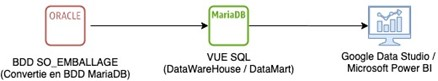
\includegraphics[scale=1]{images/solution_b.jpg} 
	\captionof{figure}{Schéma de la solution alternative proposée}
\end{center}  

\subsection{Choix de la solution}  

Nous avons donc fait le choix d’implémenter la solution A pour démontrer l’étendu des possibilités qui s’offre à SO-EMBALLAGE. Pour ce faire, nous avons converti la base de données Oracle en base de données MariaDB, puis à l’aide d’un script écrit en Javascript nous récupérons les données dans ce schéma de données, nous les modifions et nous les injectons dans un second schéma de données faisant office de Datawarehouse : « SO$\_$WAREHOUSE ». C’est sur ce schéma que nous connectons Google Data Studio pour visualiser des tendances.   

La conception d’un Datawarehouse peut être réalisée par le biais de trois modèles : 
\begin{itemize}[label=\textbullet, font=\LARGE \color{listGreen}]
	\item Le modèle en étoile 
	\item Le modèle en flocon de neige 
	\item Le modèle en galaxie 
\end{itemize} 

Ces modèles comportent deux composants : les dimensions et les faits.  Lors de la conception de modèles de données (MCD/MLD), les notions de tables et relations sont mises en avant. Néanmoins, au sein de l’informatique décisionnelle, les termes de dimensions et faits les remplacent. 

Une dimension est un axe sur lequel nous souhaitons réaliser une analyse. Un fait est une table sur laquelle portera l’analyse en question et qui reflète l’état de l’entreprise de par ses données opérationnelles.   

Notre solution actuelle contient le Datawarehouse SO$\_$WAREHOUSE, solution contenant un total de quatre tables en l’état présent. De ce fait, nous nous rapprochons du modèle en étoile sans pour autant l’atteindre car il nous faudrait améliorer notre conception et basculer toutes les clés vers une table de fait, dans notre cas la table \textit{SITE}, qui nous permet actuellement d’étudier les caractéristiques des produits et des stocks. Notre nombre de tables étant bas, il n’est pas nécessaire de partir sur un modèle en flocon de neige. Notons enfin que nous n’évoquons pas le modèle en galaxie car celui-ci est de fait, le moins pratiqué en entreprise. Ainsi, en améliorant notre conception, il serait possible pour la société d’envisager des analyses concernant les stocks et tendances sur plusieurs sites. Notre solution actuelle demeure principalement axée sur les produits et stocks. Notons que la conception devrait idéalement refléter les 3V \footnote{Volume, Vitesse, Variété: Combinaison utilisée afin de traiter des volumes de données conséquentes.} du Big Data afin d'être au top de la performance.   



\vertspace

Les tendances permettront à toute ressource en besoin de consultation (manager, directeur, analyste, CFO, RH) d’être le plus à même de prendre des décisions concernant les critères de leur système d’information. L’objectif final de notre POC (Proof Of Concept) est d’apporter à SO-EMBALLAGE les outils qui lui octroieront la force de frappe pour rester leader du marché tout en modernisant ses mécaniques internes (travail managérial, travail d’ingénierie informatique...).  

\subsection{Les indicateurs proposés}

Pour vous présenter un POC de notre solution, nous avons fait le choix de nous axer sur des indicateurs qui reflètent les problématiques de SO-EMBALLAGE et qui sont les indicateurs suivants :

\begin{itemize}[label=\textbullet, font=\LARGE \color{listGreen}]
	\item Le total des commandes par mois sur une année 
	\item Les références produit les plus vendus par mois 
	\item Les quantités restantes des produits en stock. 
\end{itemize} 

\subsection{Démonstration des résultats obtenus}

\begin{center}
	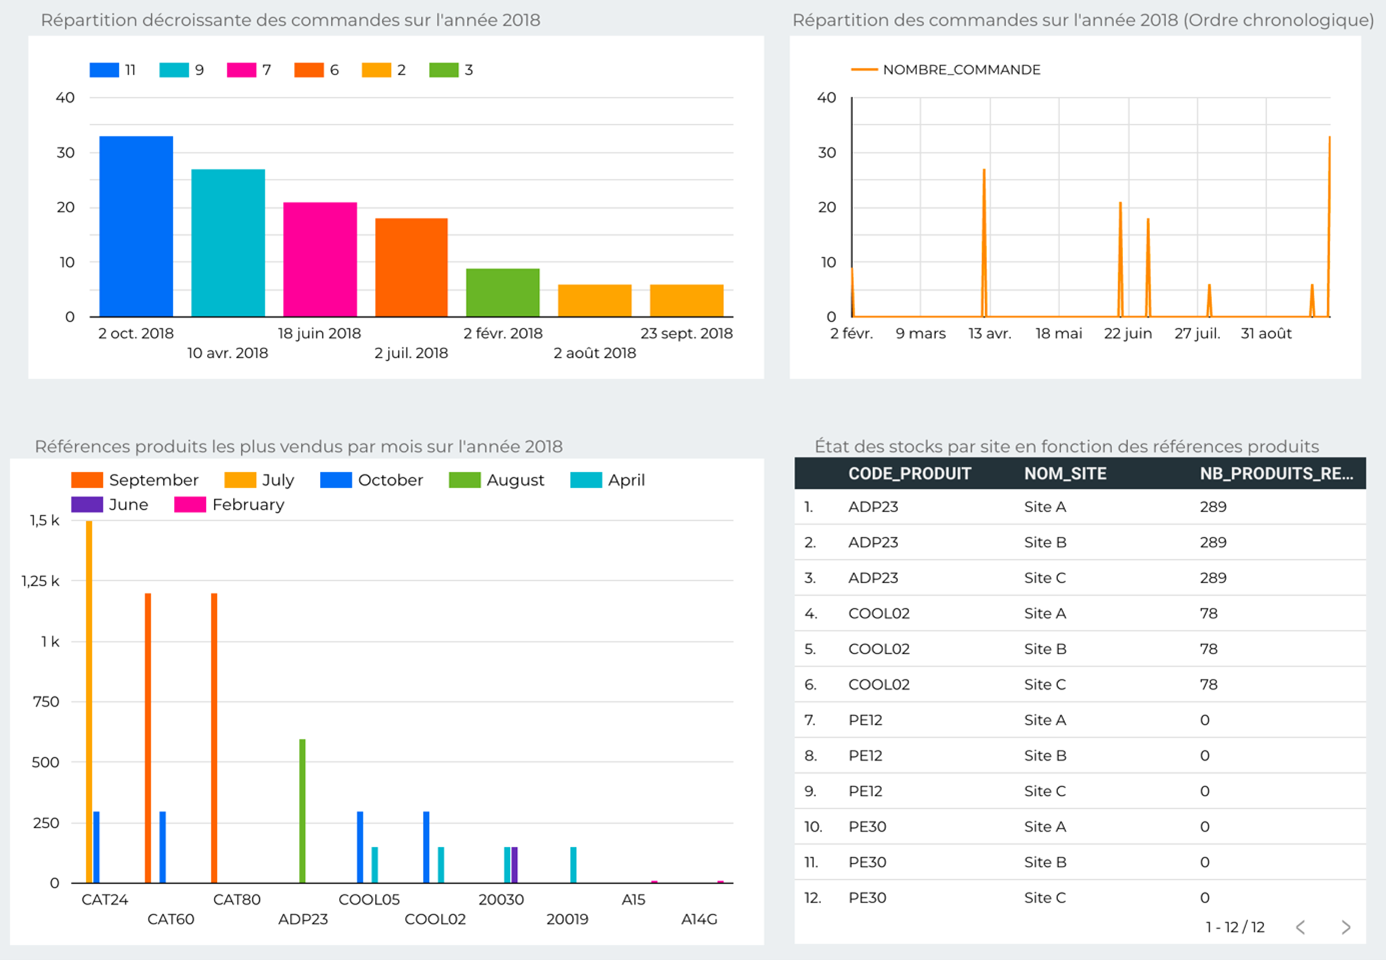
\includegraphics[scale=0.88]{images/dashboard.png} 
	\captionof{figure}{Dashboard créés à l'aide de Google Data Studio}
\end{center}  

La figure 6 montre les représentations graphiques que nous avons mises en place. Elles nous permettent d’entre-apercevoir les possibilités qui s’offrent à la société SO-EMBALLAGE avec une mise en place de ces outils sur une période de temps plus importante. 

Les deux premiers graphes nous permettent d’établir des tendances des ventes sur une année pour alimenter les stocks en conséquence au moment opportun. Le troisième schéma nous permet de visualiser les références produit les plus vendus par mois, nous pouvons ainsi éviter des problématiques de « sur-stock » sur des références qui se vendent moins. Enfin, le dernier tableau nous permet de suivre numériquement les stocks de l’entreprise par référence.  

En fonction de l’agrandissement des stocks et des espaces de stockages, il sera facile d’implémenter un suivi par entrepôt à ce niveau.   

\subsection{Alimentation du DataWareHouse}

Le data warehouse est alimenté via plusieurs sources. Tout d'abord, les données produites par SO EMBALLAGE sont envoyées à l'ETL de façon régulière. Ceci est commandé par une Cron task sur une base journalière et durant la nuit afin de ne pas charger les serveurs de base de données durant les heures de travail. Celle-ci est configurable afin de changer l'heure de l'envoi. De plus il est nécessaire d'aller chercher des données venant de sources extérieures à SO EMBALLAGE afin d'avoir une vue globale du marché sur nombre de points différents. Cette tâche est faite manuellement sur une base trimestrielle, il n'est pas nécessaire de subir cette charge de travail supplémentaire plus régulièrement afin d'avoir une bonne vision de l'état du marché actuel. Ces données sont à récupérer dans un certain format (Excel, Json, CSV, etc) et importées directement dans Google Data Studio, où les informations devront manuellement être triées. Afin de visualiser les nouvelles données, on doit finalement penser à appuyer sur le bouton “Actualiser”. 

\subsection{Préconisations}

Tout d’abord, il est important de mentionner que l’état des lieux et la structure de la base de données actuelle SO-EMBALLAGE (SGBD Oracle) ne permet pas une utilisation optimale du SI permettant entre-autre une gestion des stocks correcte. Il apparaît donc important de revoir la base de données ainsi que les processus d’alimentation de celle-ci.  

Une fois fait, nous pourrons accompagner SO-EMBALLAGE dans la mise en place d'une solution plus pérenne d'analyse et d'exploitation des données. Pour ce faire, nous pouvons recommander les solutions suivantes:

\begin{itemize}[label=\textbullet, font=\LARGE \color{listGreen}]	
	\item Utiliser la Suite Elastic comme recommandé initialement : Cette option est très intéressante car la suite ELK, malgré son arrivée relativement récente sur le marché, remplit tout à fait les besoins d’informatique décisionnel et peut supporter un large volume de données.  
	\item Une alternative d’implémentation par le biais de scripts (R, Python, Javascript...) qui feraient office d’ETL grâce aux librairies présentes dans ces technologies. Python possède des librairies fondées sur des wrappers C/C++ procurant plus de performance lors d’exécutions de scripts. Quant à R, il existe des librairies natives ainsi que le package Shiny, très simple de prise en main et permettant d’implémenter des interfaces web. Une étude sur les performances serait à réaliser car il faut considérer la volumétrie grandissante des bases de données. 
	\item L’utilisation de l’outil Talend Data Quality Studio pour la mise en place de critères de qualité des données et l’utilisation d’algorithmes et de calculs statistiques. 
	\item L’utilisation d’outils fournis par les leaders du marché en matière de solution d’informatique décisionnel tel que Talend ou Microsoft Power BI. L’avantage pour Microsoft Power BI se trouve dans sa facilité de prise en main ainsi que les nombreuses fonctionnalités proposées dans la version gratuite. De plus, il peut être apprécié pour tout afficionado du logiciel Excel car il fonde ses calculs et génération de tableau sur les tableaux dynamiques croisés d’Excel. Les montées en compétence pour ce type d’outil serait moindre et le coût engagé serait réduit. 
\end{itemize} 

Enfin, une dernière préconisation que nous souhaiterions faire auprès de SO-EMBALLAGE serait de coupler la solution BI que nous proposons avec une solution orientée Big Data. En effet, les indicateurs pourraient être utilisés afin d’effectuer des calculs statistiques et de la prédiction afin d’accompagner la direction de la société dans sa prise de décision.  

\newpage

\section{Sources}

https://www.packplus.in/ 

https://www.jpi.or.jp/english/ 

https://www.canr.msu.edu/packaging/research/ 

https://www.transparencymarketresearch.com/packaging-market-reports-35.html?page=2 

https://syskevasia-expo.gr/en/ 

\newpage

\section*{Annexes}

Script de création du Data Warehouse après étude de l'équipe.

\begin{center}
	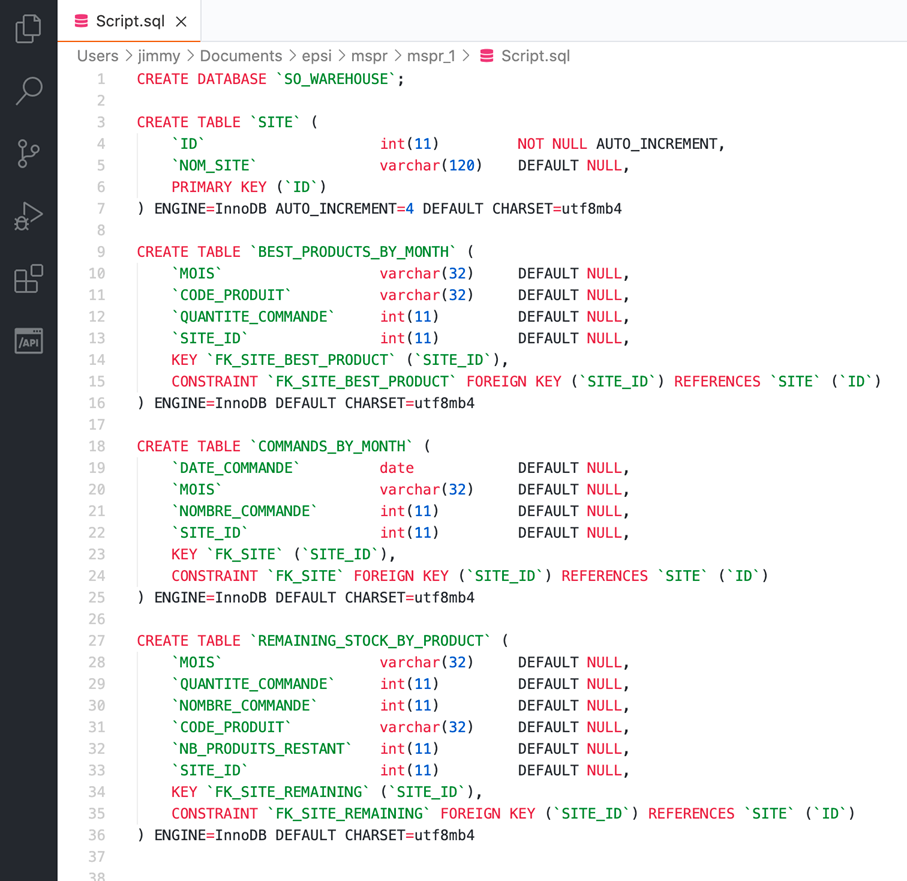
\includegraphics[scale=0.85]{images/script.png} 
	\captionof{figure}{Script SQL de génération du Data Warehouse}
\end{center}  




\end{document}